%\documentclass[]{article}
\documentclass[12pt]{article}

% my modifications:
\usepackage{fontspec}
\usepackage{booktabs}
\defaultfontfeatures{Ligatures=TeX}
\setsansfont{Calibri}
\setmonofont{Inconsolata}
\setmainfont{Linux Libertine}
\DeclareTextCommandDefault{\nobreakspace}{\leavevmode\nobreak\ }
\widowpenalty=1000
\clubpenalty=1000
\usepackage{setspace}
\onehalfspacing

% A bit bigger than one inch margins:
%\topmargin -1.43cm
%\oddsidemargin 0.4cm
%\evensidemargin 0.4cm
%\textwidth 14.5cm
\textheight 22.5cm

%\usepackage[left=1.5in,top=1.5in,right=1.5in,bottom=1.5in,nohead,nofoot]{geometry}
\usepackage{geometry}
\geometry{letterpaper}

\usepackage[round]{natbib}
\bibliographystyle{cjfas}
\bibpunct{(}{)}{;}{a}{}{;}

%\usepackage[T1]{fontenc}
%\usepackage{lmodern}
\usepackage{amssymb,amsmath}
\usepackage{ifxetex,ifluatex}
\usepackage{fixltx2e} % provides \textsubscript
% use upquote if available, for straight quotes in verbatim environments
%\IfFileExists{upquote.sty}{\usepackage{upquote}}{}
%\ifnum 0\ifxetex 1\fi\ifluatex 1\fi=0 % if pdftex
  %\usepackage[utf8]{inputenc}
%%\else % if luatex or xelatex
  %\usepackage{fontspec}
  %\ifxetex
    %\usepackage{xltxtra,xunicode}
  %\fi
  %\defaultfontfeatures{Mapping=tex-text,Scale=MatchLowercase}
  %\newcommand{\euro}{€}
%%%%%\fi
% use microtype if available
%\IfFileExists{microtype.sty}{\usepackage{microtype}}{}
%%%\usepackage{natbib}
%\bibliographystyle{plainnat}
%%%%%\usepackage{graphicx}
% We will generate all images so they have a width \maxwidth. This means
% that they will get their normal width if they fit onto the page, but
% are scaled down if they would overflow the margins.
%\makeatletter
%\def\maxwidth{\ifdim\Gin@nat@width>\linewidth\linewidth
%\else\Gin@nat@width\fi}
%\makeatother
%\let\Oldincludegraphics\includegraphics
%\renewcommand{\includegraphics}[1]{\Oldincludegraphics[width=\maxwidth]{#1}}
%\urlstyle{same}  % don't use monospace font for urls
\setlength{\parindent}{0pt}
\setlength{\parskip}{6pt plus 2pt minus 1pt}
\setlength{\emergencystretch}{3em}  % prevent overfull lines
%
\title{Portfolio prioritization of salmon conservation}
\author{Sean Anderson}
\date{}

\begin{document}
\maketitle

\section{Abstract}

First part is copied from what I wrote before (introduction and
questions). Second part outlines the simulation. I haven't yet worked
very much with the portfolios themselves, but I've set up the structure
of the simulation. I outline how the simulation is currently working and
show examples of some of the plotting functions I have to look at
simulation and portfolio optimization.

\section{Introduction}

{[}Based partly on Jon's notes.{]} Managing risk is fundamental to the
conservation of an endangered species. When an endangered species exists
as a metapopulation, we can manage risk at two levels: at the population
level or at the metapopulation level. Typically we treat sources of risk
at the metapopulation level as external and uncontrollable and so we
manage risk by altering anthropogenic disturbances such as fishing or
hunting on a population level as well as improving connectivity of
populations.

The management of financial portfolios provides another way of
considering risk. Economists consider the risk and performance of a
financial portfolio as depending on the weighting of individual assets
that make up the portfolio. Modern Portfolio Theory (MPT) proposes that
there is a set of portfolios that achieves maximum expected return for a
level of expected risk or minimum expected risk for a level of expected
return \citep{Markowitz1952, Markowitz1959}. This optimal set contains
portfolios that range along a continuum of risk-tolerance; economists
refer to this set as the efficient frontier.

Similarly, expected growth rate and variance at a metapopulation level
will be a function of the properties of the populations. A portfolio
approach to managing risk for a metapopulation therefore considers how
conservation might affect the
\texttt{weight'' of each population in the metapopulation}portfolio''.

Bring in salmon: we can manage risk at the population level or at the
ESU level. ESU-level conservation is mandated but we generally lack
tools to quantitatively manage risk at this level.

\begin{table}[h!]
\centering
\small
\caption{Components of salmon metapopulation portfolios}
\begin{tabular}{p{3.6cm}p{7.5cm}}
\toprule
Component & Definition for the salmon portfolio\\
\midrule
Assets & Viable salmonid populations? Stream-level populations? Depends on the 
system\\
Portfolio & The salmon metapopulation; possibly an ESU\\
Portfolio managers & Salmon managers\\
Investors & Salmon managers, conservation agency, or salmon fishers (each with 
their own goals and mandates)\\
Asset weights & Carrying capacity, or catches, or salmon spawner (or return) 
abundance\\
Asset returns & Annual rate of change of salmon returns or spawners; possibly 
annual rate of change of fisheries catches\\
Asset risk & Could be variance of asset returns; could be a coherent asymmetric 
risk metric such as CVaR\\
\bottomrule
\end{tabular}
\label{tab:port-components}
\end{table}

\subsection{Portfolio prioritization of salmon conservation}

Here, we conduct a post-hoc assessment of the set of optimal salmon
portfolios given various return-risk definitions and objectives. We ask:
What does a portfolio approach to management tell us about salmonid
conservation priorities? Does it produce any rules of thumb about what
optimal portfolio management of salmonid metapopulations would entail?

\subsection{Questions}

\begin{enumerate}
\def\labelenumi{\arabic{enumi}.}
\item
  What are the attributes of the populations that form the optimal set?
  For example, are populations with high response diversity prioritized?
\item
  How much lower is stream-level and ESU-level extinction risk for the
  optimal portfolios than the less optimal portfolios? Extinction
  probability could be estimated through long-term simulation or through
  an asymmetric risk metric like conditional value at risk (CVaR). Given
  I am including straying, this will most likely be a
  quasi-extinction-risk metric.
\item
  How do our answers to other questions change depending on what we
  measure on the risk-return axes? For example, we could trade off the
  mean rate of change of salmon returns vs.~variance of the rate of
  change. This would be most similar to a financial portfolio
  optimization. We could also trade off the salmon returns (or catches)
  themselves. Further, we could work with variance or a downside risk
  metric like CVaR.
\item
  How do constraints (e.g.~viable salmonid population (VSP)-like
  constraints) affect the selected portfolios in risk-return space and
  in terms of common metrics such as population-level and ESU-level
  extinction risk?
\item
  How do the properties of the optimal portfolio set change based on
  different kinds of environmental driver patterns? For example,
  magnitude of driver variance, cyclical dynamics like the PDO, black
  swans or unexpected surprises, increases in temperature and
  variability through time (climate change).
\end{enumerate}

\section{Simulation}

See Figure \ref{fig:sim-diagram} for an illustration of the simulation
structure.

\begin{figure}[htbp]
  \centering
    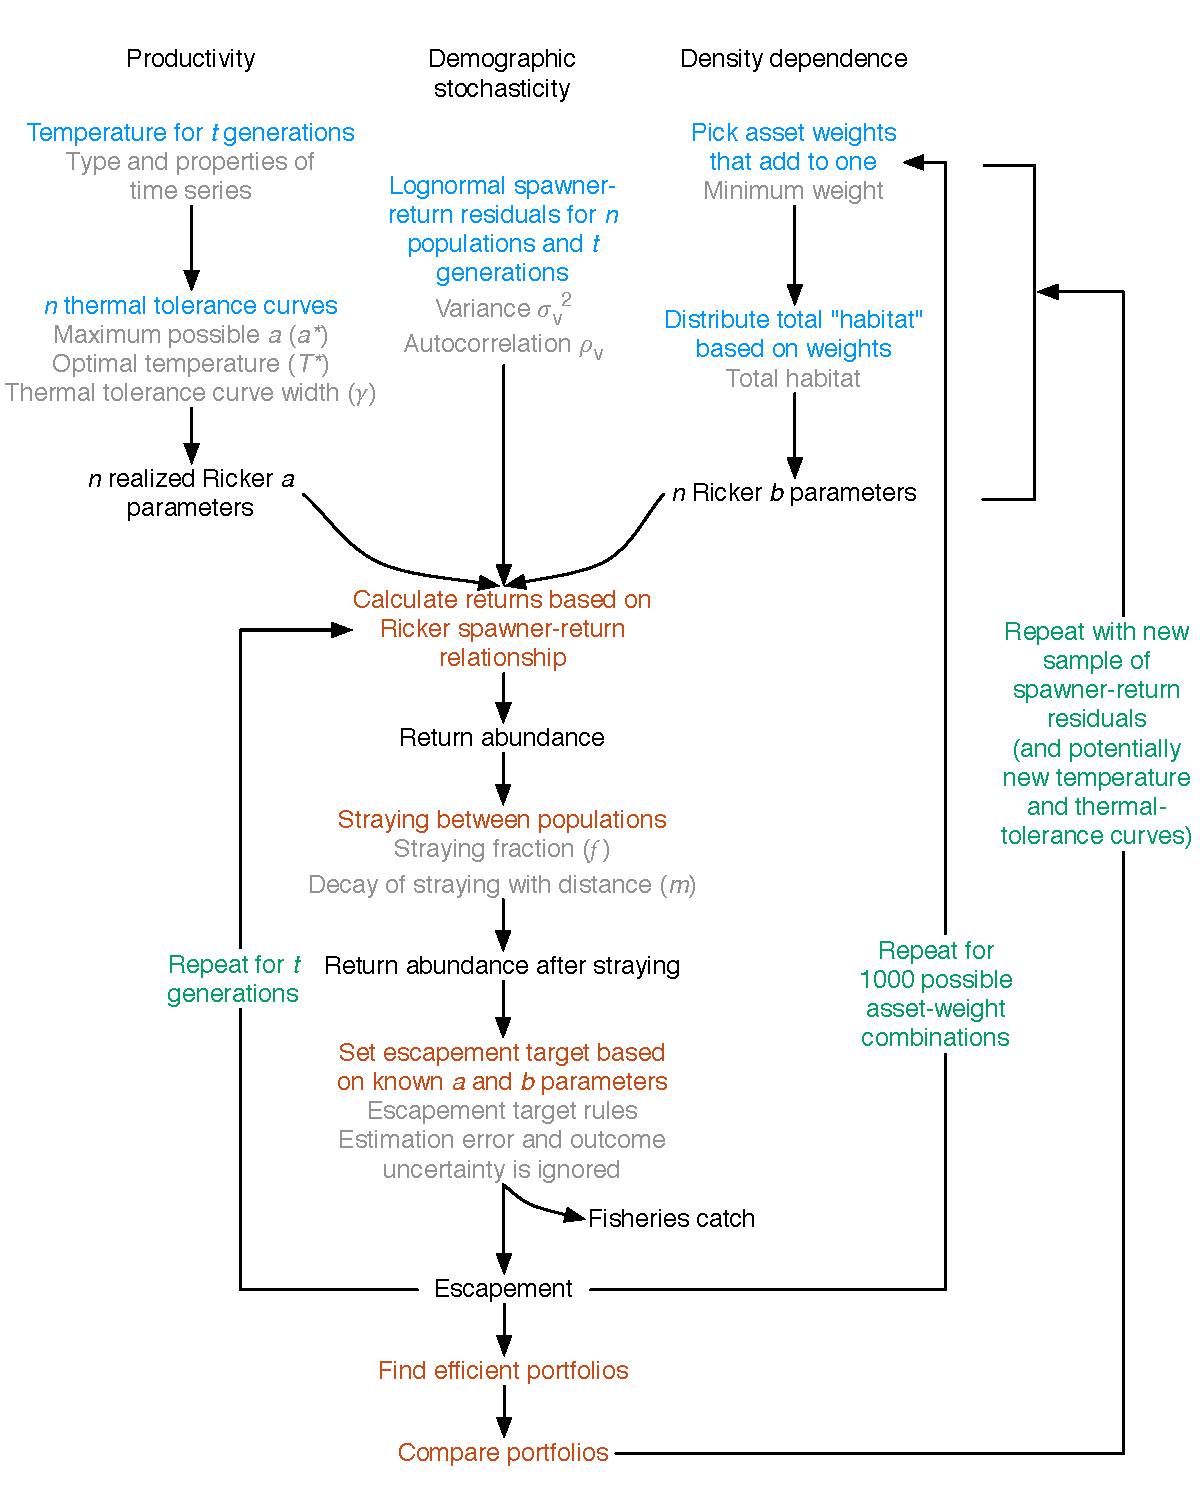
\includegraphics[height=7in]{simulation_diagram.pdf}
 \caption{Flow chart of the salmon-metapopulation simulation and portfolio optimization. There are $n$ salmon populations and $t$ generations. Blue text indicates values that are generated before the simulation progresses through time. Orange text indicates steps in which calculations are performed. Black text indicates values that are calculated. Grey text indicates parameters that can be set. Green text indicates the looping structure of the simulation.}
  \label{fig:sim-diagram}
\end{figure}

\subsection{Spawner-return relationship}

I am using a Ricker curve,

\begin{equation}
R_{ti} = S_{ti}e^{a_{ti}(1-S_{ti}/b_i) + w_{ti}},
\end{equation}

\noindent
where $t$ represents a generation time, $i$ represents a population, $R$
is the number of returns, $S$ is the number of spawners, $a$ is the
productivity parameter (which can vary with the environmental signal),
and $b$ is the density-dependent term (which is used as the asset
weights in the portfolios). The term $w_{ti}$ represents first-order
autocorrelated error (AR1). Formally, $w_{ti} = w_{ti-1} \rho + v_{ti}$,
where $v_{ti}$ represents independent and normally distributed error
with mean 0 and standard deviation of $\sigma_v$. The parameter $\rho$
represents the correlation between residuals from subsequent years.

\subsection{Escapement targets}

I am calculating spawning abundance MSY $S_{MSY}$ each generation using
the equation $S_{MSY} = b(0.5-0.07a)$ from \citet{Hilborn1992} p272,
Table 7.2. I am using the precisely known $a$ and $b$ values each time
and assume perfect implementation of the escapement goal (no outcome
uncertainty) and no upper limit on how much the fishery can harvest. We
may want to add a bit of noise here, say by assuming a constant value
for $a$ or adding some implementation uncertainty. We need some level of
harvesting to keep the spawning population away from carrying capacity.
At carrying capacity, the productivity parameter $a$ has minimal effect
on population dynamics, making it a poor way to integrate response
diversity.

\subsection{Environmental signal}

I have programmed five different kinds of environmental signals. I think
it's easiest to think of these as temperature signals, but they could
represent more general environmental anomalies, such as the PDO. The
five kinds of environmental signals are described in Table
\ref{tab:env-types} and illustrated in Figure \ref{fig:env-ts}. Later, I
may include black-swan-like events, although the regime shifts could be
seen this way if the changes are dramatic enough. So far all figures use
a sine wave. The problem with using a randomly generated ARMA time
series is that you get much greater differences in the portfolios from
run to run.

\begin{table}[h!]
  \centering
  \small
  \caption{Environmental signals, parameters, and descriptions.}
\begin{tabular}{p{3.2cm}p{3.25cm}p{6.8cm}}
\toprule
Signal type & Parameters & Description \\
\midrule
Sine wave & $\overline{T} + A \cdot \sin(\omega t + \phi)$& $\overline{T}$ is 
the mean environmental value, $A$ is the amplitude, $\omega$ is the frequency in 
radians, and $\phi$ is the phase\\
ARMA & AR1, MA1, $\sigma_T$ & First-order autoregressive (AR1) and moving 
average (MA1) parameters and standard deviation; mean is assumed to be 0\\
Regime shifts & $T_{b0},T_{b1}, \ldots, T_{bn}$; $T_{v0},T_{v1}, \ldots, T_{vn}$ 
& Breakpoints ($T_{b}$) and values ($T_v$) for regimes $1$ through $n$\\
Linear change & $T_{\mathrm{min}}$, $T_{\mathrm{max}}$ & Minimum and maximum 
values\\
Constant & $T_{\mathrm{constant}}$& Constant value\\
\bottomrule
\end{tabular}
\label{tab:env-types}
\end{table}

\begin{figure}[htbp]
\centering
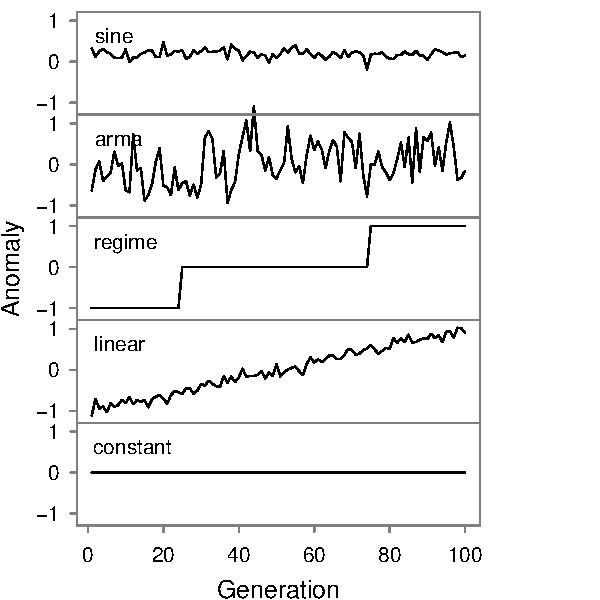
\includegraphics{figure/env-ts.pdf}
\caption{Example temperature time series\label{fig:env-ts}}
\end{figure}

\subsection{Straying}

{[}Insert a bit here about my research on straying and it's influence on
metapopulation dynamics for salmon{]}. Essentially, straying should be
enough to prevent local extinctions and ensure all possible habitat is
occupied, but probably not strong enough to noticeably affect population
dynamics or synchrony \citep{Schtickzelle2007}.

I've implemented straying as in \citet{Cooper1999}. I generate a matrix
that represents the fraction of straying between any two populations. I
have set up the metapopulation (thus far) as in in a very simple
scenario: the populations are arranged in a line and those that are
nearer to each other are more likely to stray between each other
{[}insert caveats{]}. Two parameters control the straying: the fraction
of fish that stray from their natal stream in any given generation $f$
and the rate at which this straying between streams decays with distance
$m$. I calculated the number of salmon straying from stream $i$ to
stream $j$ as,

\begin{equation}
  \mathrm{strays}_{tij} = \frac{S_{ti} f e^{-m \lvert i-j \rvert }}{\sum\limits_{k \neq j}^{} e^{-m \lvert k-j \rvert }},
\end{equation}

where the denominator is a normalization constant to ensure that no
salmon are gained or lost. The subscript $k$ represents a stream ID.
{[}Not sure this is written correctly --- I'll think about it --- but it
should be coded correctly.{]} There is no straying from and to the same
stream. See Figure \ref{fig:stray-matrix} for an example straying
matrix.

\begin{figure}[htbp]
\centering
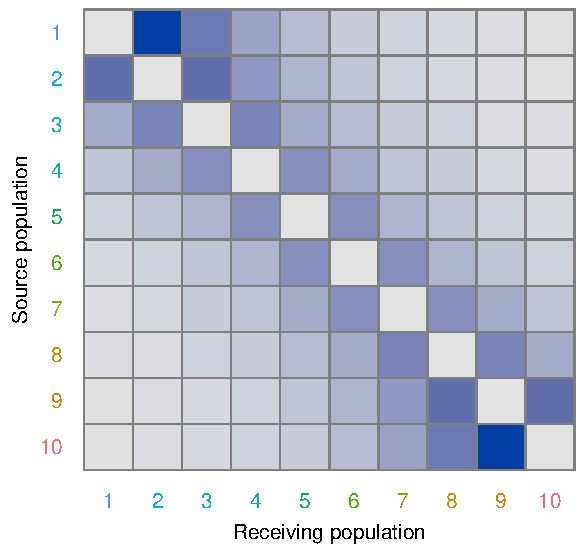
\includegraphics{figure/stray-matrix.pdf}
\caption{Example straying matrix. Darker blue colours indicate a greater
rate of straying.\label{fig:stray-matrix}}
\end{figure}

\subsection{Diversity of response to the environmental conditions}

{[}insert research I've done here on what can generate diversity of
response to the environment across populations and how it is typically
incorporated{]} This is a critical part to the paper.

I am incorporating diversity of response to environmental conditions,
say temperature, via changes in the Ricker $a$ parameter. I am using
thermal tolerance curves, based loosely on \citet{Eliason2011}. They
identify unique thermal tolerance curves in terms of cardiorespiratory
performance. I am using approximately the same temperature ranges and
variability of those curves, but applying them to productivity. I show
the curves I'm currently using in Figure \ref{fig:thermal-curves}. We
could vary the distribution of the optimum temperatures, the maximum $a$
values, and the width of the curves if we wanted, although I think the
current curves are a simple and straightforward base scenario and we may
not need to do anything more complicated.

I calculate $a_{ti}$, the realized Ricker productivity parameters after
accounting for thermal tolerance, as

\begin{equation}
  a_{ti} = a_i^* + \gamma_i (T_t - T_i^*)^2,
\end{equation}

where $a_i^*$ is the maximum possible productivity parameter for
population $i$, $T_t$ is the temperature at time step $t$, $T_i^*$ is
the optimal temperature for population $i$, and $\gamma_i$ controls the
width of the thermal tolerance curve for each population. See Figure
\ref{fig:thermal-curves} for the default thermal tolerance curves for
ten populations.

Another possibility would be to draw the $a^*$, $\gamma$, and $T^*$
randomly. The advantage to setting it up as I have (with pre-specified
thermal tolerance curves) is that it will hopefully make the post-hoc
analysis of what affects the efficient frontier weights more
straightforward.

\begin{figure}[htbp]
\centering
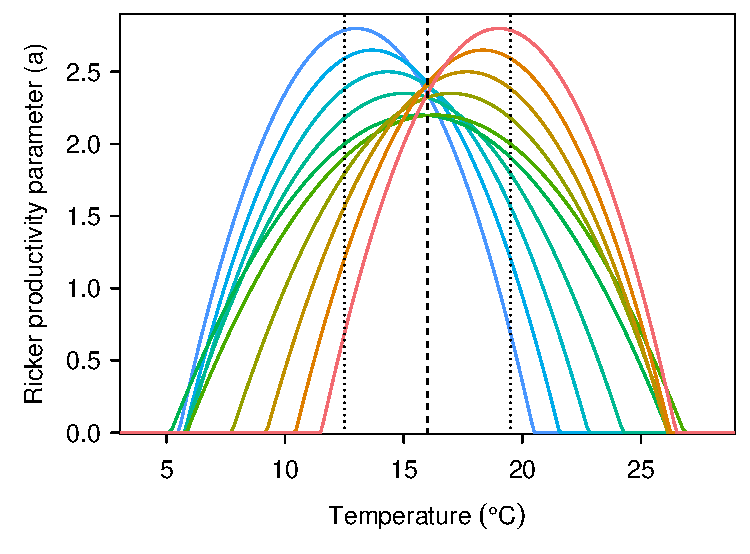
\includegraphics{figure/thermal-curves.pdf}
\caption{Thermal tolerance curves for ten populations. Here, and
throughout this document, I have used the same rainbow of colours to
identify the salmon populations. The populations are arranged from blue
(more productive with cooler temperatures) to red (more productive with
warmer temperatures\label{fig:thermal-curves}}
\end{figure}

\section{Portfolio optimization}

Details to follow. Quick version: I Monte Carlo the $b$ parameters (with
a specified minimum value) and measure the resulting mean and variance
of the rate of growth of the metapopulation salmon returns. I then
identify the set of $b$ parameters (i.e.~the set of weights) that
results in the efficient frontier. We could later choose to work with
risk metrics like conditional value at risk (CVaR), which measure the
probability of a ``bad'' event specifically, not the symmetrical
variance.

To find the efficient portfolios I divide all portfolios into bins by
mean rate of change and find the portfolios with the minimum variance
within each bin. I discard all portfolios with a mean rate of change
below the minimum variance portfolio. These are ``undesirable''
portfolios.

\section{Comparing portfolios}

This is a big area to think about. How do portfolios differ along the
frontier? How do the frontier portfolios differ from non-frontier
portfolios? What is the best way to visually compare them? What aspects
to compare? Are there summary statistics we could use to compare them?

\section{Some sample simulations}

The following are options and their default values:

\begin{verbatim}
  n_t = 120, # number of years
  n_pop = 10, # number of populations
  stray_decay_rate = 0.3, # rate that straying decays with distance
  stray_fraction = 0.01, # fraction of fish that stray from natal streams
  b = rep(1000, n_pop), # Ricker density-dependent parameter
  spawners_0 = round(b), # spawners at start
  sigma_v = 0.1, # stock-recruit residual SD
  v_rho = 0.4, # stock-recruit residual AR1 correlation
  a_width_param = rep(0.02, n_pop), # width of thermal curves by pop
  optim_temp = seq(13, 19, length.out = n_pop), # optimal temperatures by pop
  max_a = rep(1.4, n_pop), # maximum Ricker a values by pop at optimum temp
  env_type = c("sine", "arma", "regime", "linear", "constant"),
  env_params = list(amplitude = 2.0, ang_frequency = 0.2, phase = 0, mean_value = 16),
  use_cache = FALSE, # regenerate stochastic values? 
  add_straying = TRUE # include or ignore straying
\end{verbatim}

First, let's run a couple example simulations:

\begin{figure}[htbp]
\centering
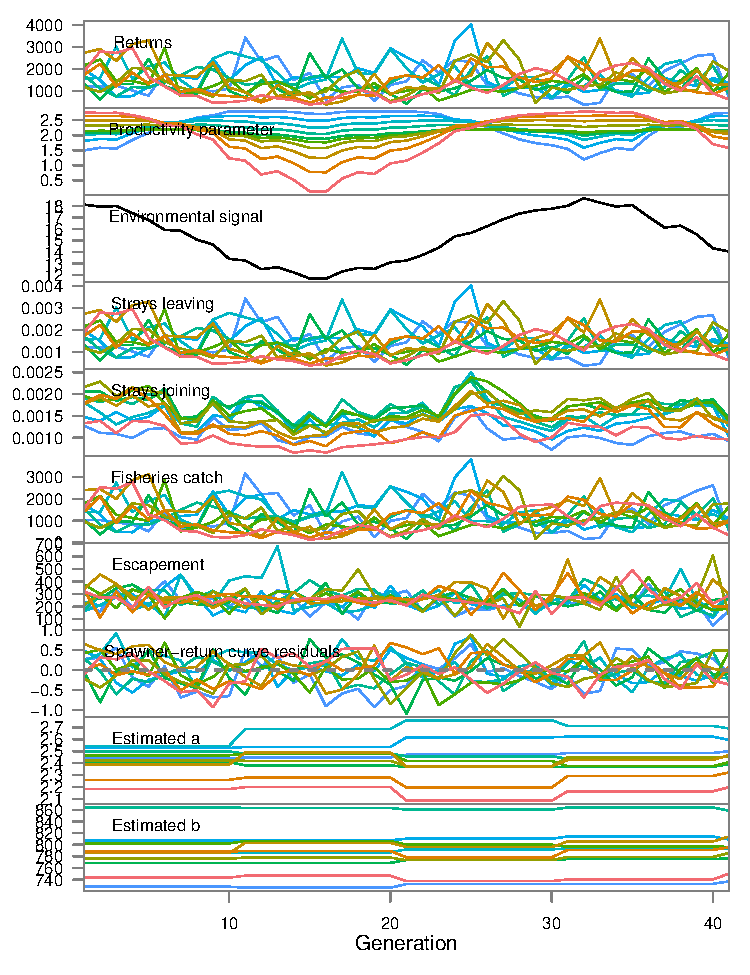
\includegraphics{figure/run-base-example1.pdf}
\caption{Example simulation with all parameters at default values. I'm
only showing a sample of 40 generations (after the burn-in period). From
top to bottom: salmon returns each generation (catch plus escapement);
Ricker $a$ parameter; the environmental signal (could think of it as
temperature or a composite environmental signal like the PDO); number of
salmon straying by population; number of straying salmon being received
by population; fisheries catch based on escapement MSY calculation;
salmon escapement; residuals from the spawner-return curve.}
\end{figure}

\begin{figure}[htbp]
\centering
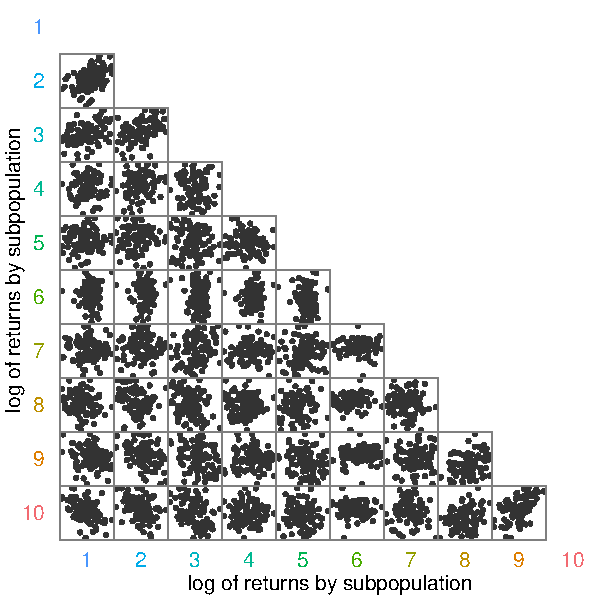
\includegraphics{figure/plot-base-corrs.pdf}
\caption{A plot comparing the log(returns) between each population. The
population colours and numbers match in all figures. Note how
populations 1 and 10 have asynchronous returns whereas populations with
more similar thermal-tolerance curves (say populations 9 and 10) have
more synchronous dynamics. Populations with thermal tolerance curves in
the middle (e.g.~population 6) are less correlated with other
populations. Their population dynamics end up primarily driven by
demographic stochasticity and less so by temperature-induced systematic
changes in productivity.}
\end{figure}

\begin{verbatim}
Error: could not find function "ricker_ar1"
\end{verbatim}

\begin{figure}[htbp]
\centering
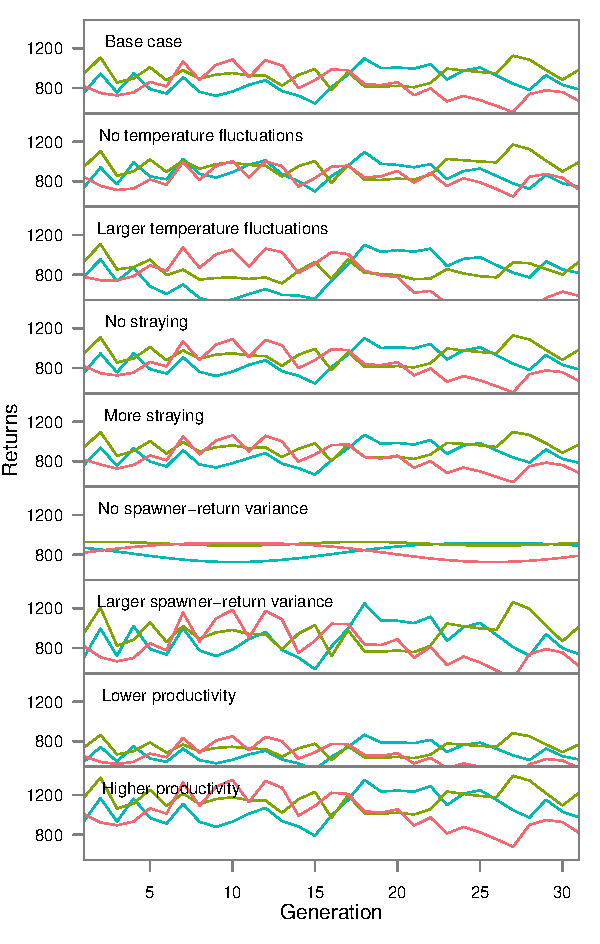
\includegraphics{figure/plot-various-options-ts-3pops.pdf}
\caption{Example simulations with different parameter values. I am
showing three populations here to make the plots easier to
interpret.\label{fig:sim-param-ts-3}}
\end{figure}

\begin{figure}[htbp]
\centering
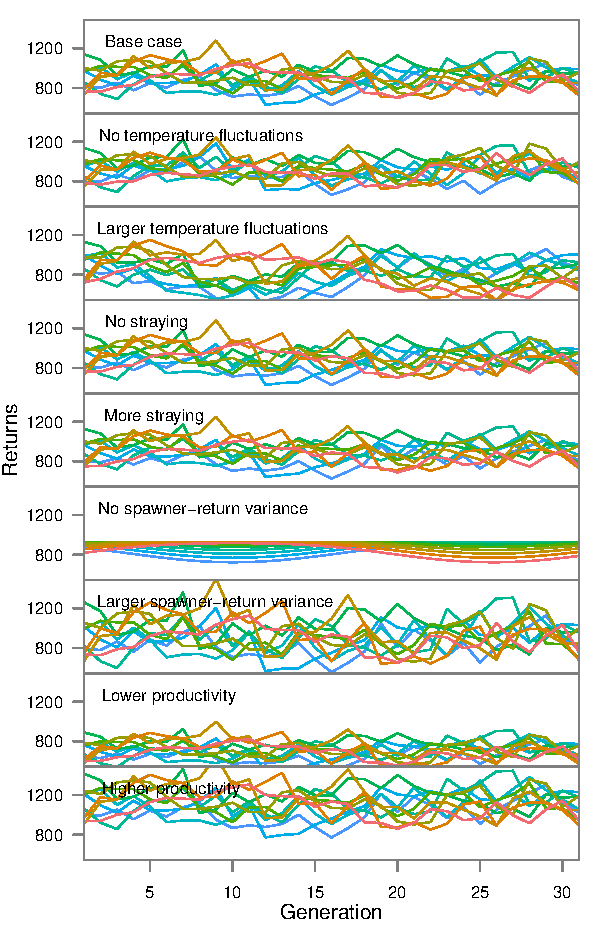
\includegraphics{figure/plot-various-options-ts.pdf}
\caption{Example simulations with different parameter values. This
version has ten populations.\label{fig:sim-param-ts-10}}
\end{figure}

\clearpage

\section{An example of portfolio optimization}

Now, let's run an example where we find the $b$ values that form the
efficient frontier of metapopulation portfolios.

\begin{figure}[htbp]
\centering
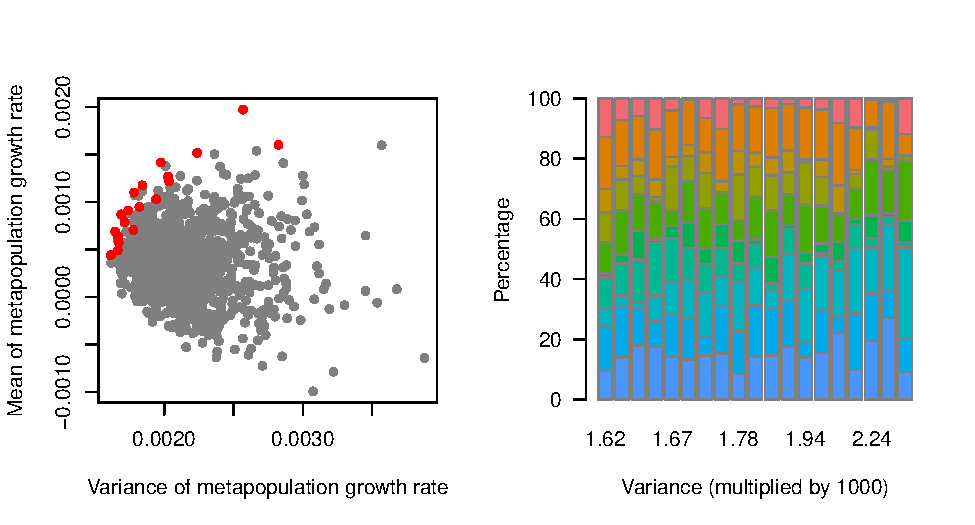
\includegraphics{figure/eff-frontier-eg.pdf}
\caption{Efficient frontier of metapopulation portfolios (red dots).
Each dot represents a different set of weights of the Ricker $b$
parameters. Metapopulation growth rate is the first difference of the
log of total metapopulation abundance. The colours in the right panel
correspond to the other figures.}
\end{figure}

\begin{figure}[htbp]
\centering
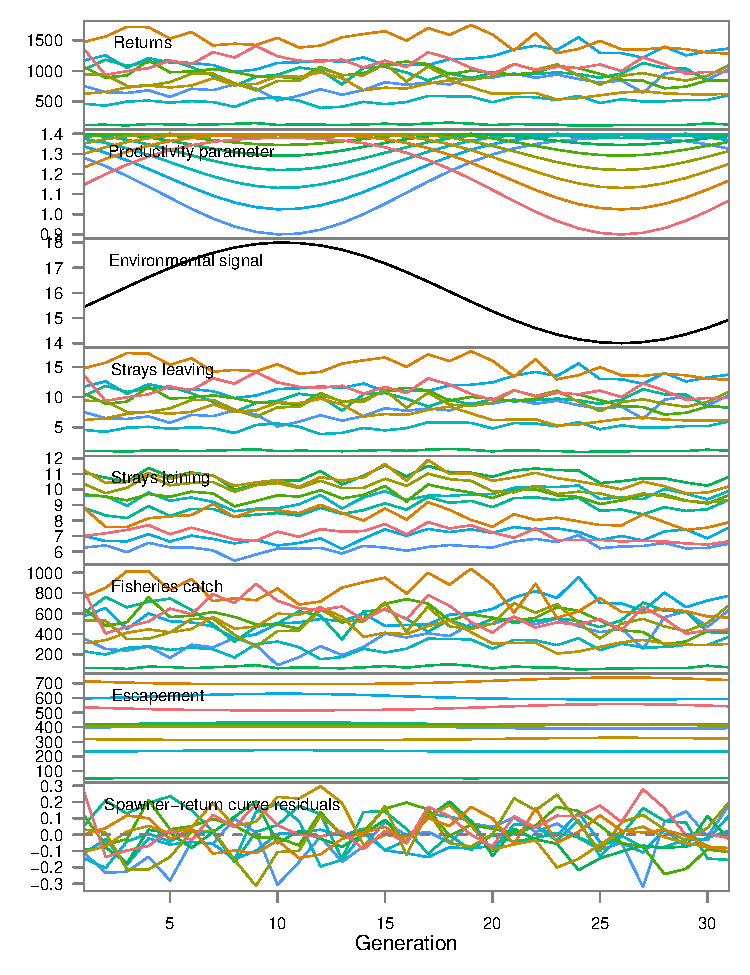
\includegraphics{figure/plot-eff-ports.pdf}
\caption{Simulation output from the minimum-variance metapopulation.}
\end{figure}

\begin{verbatim}
Error: could not find function "ricker_ar1"
\end{verbatim}

\begin{figure}[htbp]
\centering
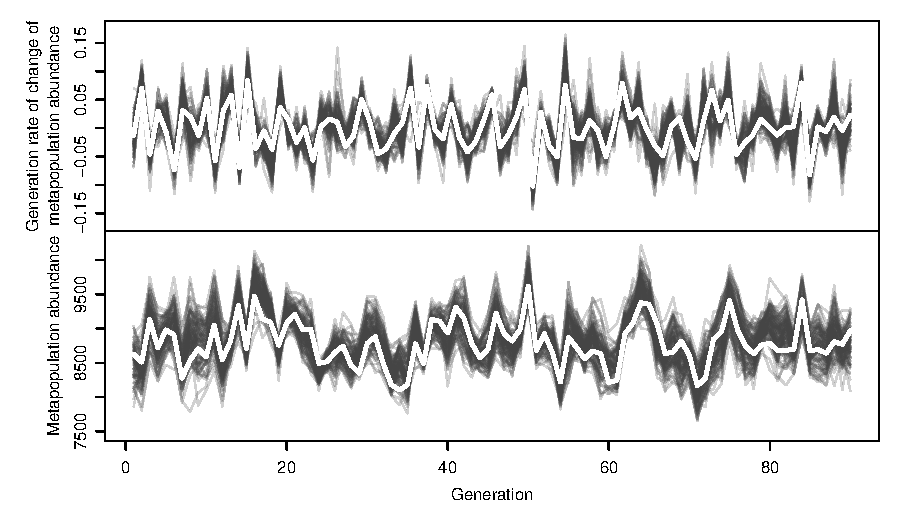
\includegraphics{figure/plot-portfolio-timeseries.pdf}
\caption{Time series for a random sample of portfolios (grey lines) and
the minimum-variance portfolio (white lines). The top panel shows rate
of change or metapopulation abundance at each time step and the bottom
panel shows the metapopulation abundance.}
\end{figure}

\clearpage

\renewcommand\refname{References}
\bibliography{jshort,salmonport}

\end{document}
